%!TEX root = Report.tex

% Overvej at kalde dette afsnit "Experimentation" eller "Testing"
% 
% vis hvornår det virker og hvornår det ikke virker. 
% Se at det virker når vi regnede med at det virkede.
% 
% Hvad tester vi?
% Hvordan tester vi det?
% Virkede det efter hensigten?
% Hvorfor/hvorfor ikke?
% Er der nok testing?
% Hvordan kan man lave mere testing?
% Er der andre måder vi kunne have testet på? (fordele og ulemper ved det)

%---->>>Vi mangler noget om hvor lang tid af gangen vi kan tracke!

\subsection{Testing the tracking software with real ants}
\label{testing}

Having solved the problem of finding an ant in a single image and integrated our software with the XY-plotter and cameras, this section focuses on testing how the solution works with a video feed of an ant moving around in a controlled environment.\\

The goal of these tests, was to test ant tracking in an environment that was as close to a real environment as possible, but still controlled enough to be able to track the ant. The tests were performed in an ordinary office environment, with the plotter placed on a table. The room was only lit by daylight, and we used the setup explained in Section \ref{sec:setup}, with a petri dish filled with dirt surrounded by water, as can be seen in Figure \ref{fig:petridish}. According to our experimentation described in Section \ref{ants} we painted our ant with a white color to have the best possible color for tracking. \\

In the following we will show several results of running the solution, both where the tracking works as intented, but also situations where the solution does not work. We will end this section with a summary of the challenges presented by this real time testing and suggest possible solutions to the problems and an overall evaluation of how the software together with the plotter and camera performs. We will also comment on the important observations made during testing.\\

We will begin by showing several images from the test where tracking works. Examples can be seen in Figure \ref{fig:ant_tracking}. We are showing both the final thresholded image, as well as the original image. For this test, we used the following values $\alpha = 2.0$ for contrasting and $T = 240$ for thresholding.\\

\begin{figure}
        \centering
        \begin{subfigure}[b]{0.35\textwidth}
                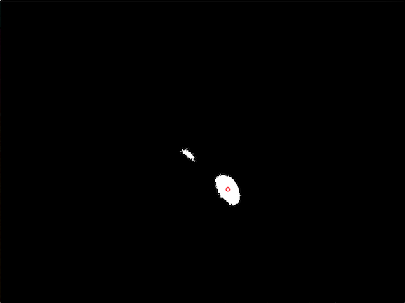
\includegraphics[scale = 0.3]{img/good1t}
                \caption{}
        \end{subfigure}
		\quad
        \begin{subfigure}[b]{0.35\textwidth}
                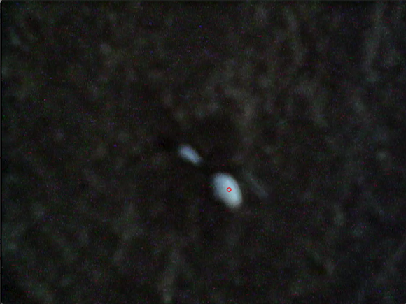
\includegraphics[scale = 0.3]{img/good1}
                \caption{}
        \end{subfigure} \hfill \\ \mbox{}\\
        \begin{subfigure}[b]{0.35\textwidth}
                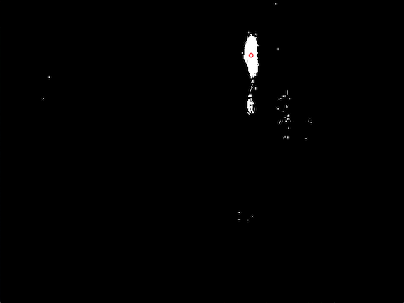
\includegraphics[scale = 0.3]{img/good2t}
                \caption{}
        \end{subfigure}
		\quad
        \begin{subfigure}[b]{0.35\textwidth}
                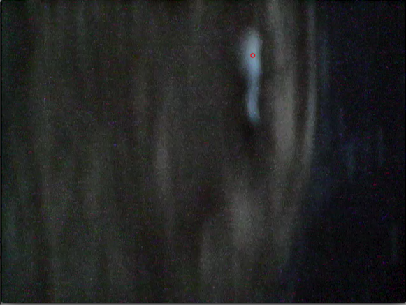
\includegraphics[scale = 0.3]{img/good2}
                \caption{}
        \end{subfigure}\hfill \\ \mbox{}\\
        \begin{subfigure}[b]{0.35\textwidth}
                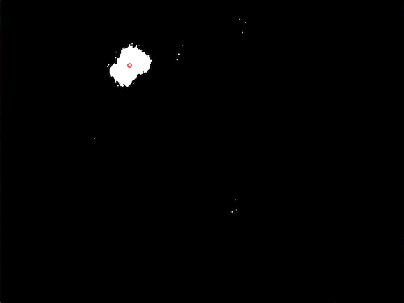
\includegraphics[scale = 0.3]{img/good3t}
                \caption{}
        \end{subfigure}
		\quad
        \begin{subfigure}[b]{0.35\textwidth}
                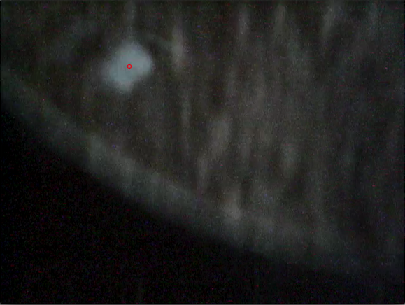
\includegraphics[scale = 0.3]{img/good3}
                \caption{}
        \end{subfigure}\\ \mbox{}\\
        \begin{subfigure}[b]{0.35\textwidth}
                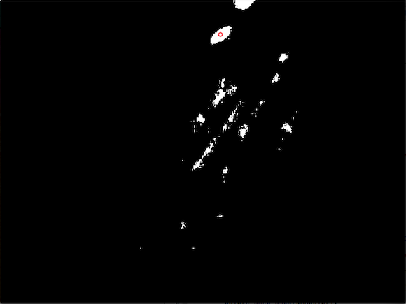
\includegraphics[scale = 0.3]{img/good4t}
                \caption{}
        \end{subfigure}
		\quad
        \begin{subfigure}[b]{0.35\textwidth}
                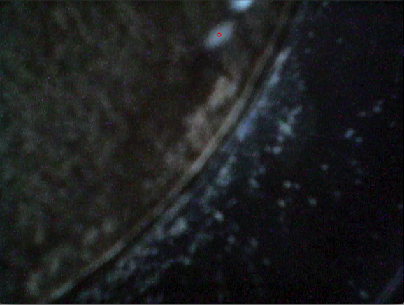
\includegraphics[scale = 0.3]{img/good4}
                \caption{}
        \end{subfigure}
		\caption{Examples of real time ant tracking.}
		\label{fig:ant_tracking}
\end{figure}

We can see from the images in Figure \ref{fig:ant_tracking} that the software is able to handle different situations where a) the image is very blurry, b) there is noise in the thresholded image and c) the ant is clearly visible. In general, we can say that it is possible to track the ant in situations where it is distinguishable from anything else in the image, or when it is the largest object present after image processing. However our tests also showed that we were unable to track the ant when certain conditions were met, as shown in Figure \ref{fig:ant_fail}.\\

\begin{figure}
        \centering
        \begin{subfigure}[b]{0.35\textwidth}
                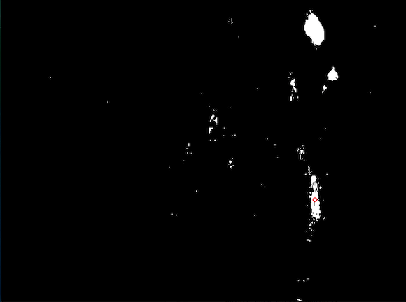
\includegraphics[scale = 0.3]{img/bad1t}
                \caption{}
        \end{subfigure}
		\quad
        \begin{subfigure}[b]{0.35\textwidth}
                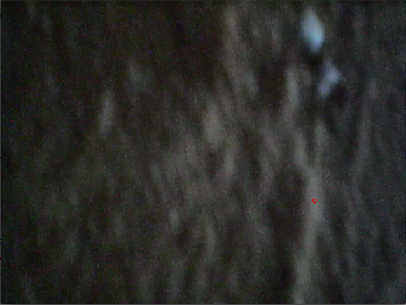
\includegraphics[scale = 0.3]{img/bad1}
                \caption{}
        \end{subfigure} \hfill \\ \mbox{}\\
        \begin{subfigure}[b]{0.35\textwidth}
                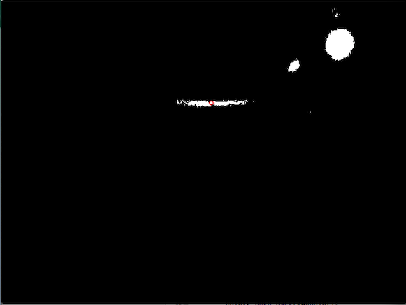
\includegraphics[scale = 0.3]{img/bad2t}
                \caption{}
        \end{subfigure}
		\quad
        \begin{subfigure}[b]{0.35\textwidth}
                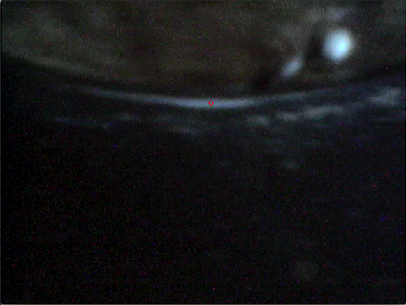
\includegraphics[scale = 0.3]{img/bad2}
                \caption{}
        \end{subfigure}\hfill \\ \mbox{}\\
        \begin{subfigure}[b]{0.35\textwidth}
                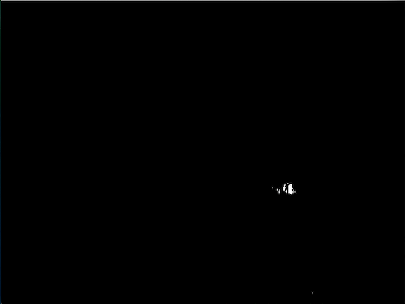
\includegraphics[scale = 0.3]{img/bad3t}
                \caption{}
        \end{subfigure}
		\quad
        \begin{subfigure}[b]{0.35\textwidth}
                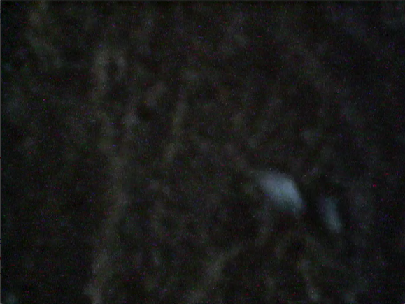
\includegraphics[scale = 0.3]{img/bad3}
                \caption{}
        \end{subfigure}\\ \mbox{}\\
        \begin{subfigure}[b]{0.35\textwidth}
                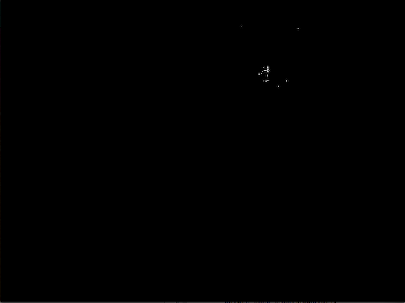
\includegraphics[scale = 0.3]{img/bad4t}
                \caption{}
        \end{subfigure}
		\quad
        \begin{subfigure}[b]{0.35\textwidth}
                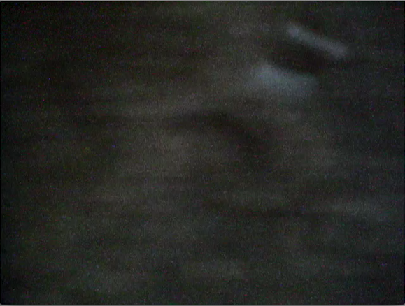
\includegraphics[scale = 0.3]{img/bad4}
                \caption{}
        \end{subfigure}
		\caption{Examples of tracking failues.}
		\label{fig:ant_fail}
\end{figure}

In image \emph{b} and \emph{d} in Figure \ref{fig:ant_fail}, tracking fails because the ant is no longer the largest object in the thresholded images \emph{a} and \emph{c}. In image \emph{b} it is because the dirt reflects too much light, and in image \emph{d} it is because the water reflects too much light. One might wonder why, especially in image \emph{c}, the ant is considered smaller than the reflection. This is because the blob detector in OpenCV, assumes blobs are \emph{circular} and the size of a blob is actually the radius of that circle. Because the blob is lengthy but slim the radius of the circle surrounding the entire blob becomes very large, and as such the radius reported by the blob detector is so as well. This leads to the problem that our software interprets the water reflection to be the largest blob in the image. \\

In image \emph{f} the problem arises because the image is too dark. Even with the given contrast, most of the white color does not exceed the threshold boundary, and the pixels that makes it past the threshold is considered noise by the blob detector. In image \emph{h} the image is simply too blurry (the ant is in the upper right corner), which makes both the ant and the white color "disappear" into the background.\\

In summary the problems found throughout our tests can be generalized to cover the following issues:

\begin{itemize}
    \item Background reflections.
    \item Bad lighting of test area.
    \item Camera blurryness.
    \item Ant speed.
\end{itemize}

To solve the issues of background reflections and lighting conditions a lab environment could be established where there would be no daylight involved, and the entire test area lit by diffuse light. We tried using the two small diodes attached to the camera to improve the lighting conditions in the image, however the light was too bright making both the ant and dirt/water appear white in the image. A proper test environment would ensure both a much better lit ant, and possibly also a solution to track an ant using other colors than white. Furthermore, reflections would not be as apparent due to the lack of a strong single light source, and would further reduce shadows from the arm of the plotter.\\

During the tests we noticed that the ants moved very fast, and every so often they would move out of the cameras view in a second or two. Most of the time the camera could keep up with the ant, but because of the speed many of the images produced by the camera were very blurry, and at some point tracking would fail because the ant could not be located in the blurry images as shown in Figure \ref{fig:ant_fail}. To solve this issue, one could use ants that moved slower, or move the camera further up from the petri dish, such that it did not have to move as much between every frame as in our case and capture a larger part of the petri dish in each frame. \\

We do not know if termites move as fast as the ants available to us. If not, then they would be easier to monitor and follow with this setup. We also noticed that the increased speed of the ants were often triggered when they were frigthened. We noticed this when painting the ants, and releasing them into the test environment. They would however slow down over time. \\

During our test, the XY-plotter would stutter from time to time, making loud noises and shake the petri dish for a brief moment. This probably caused a frightened reaction with the ant, seing as it started to move very fast, escaping the camera due to blurry images. \\
%It should be noted that putting the ants in a freezer for a couple of minutes would paralyze them, and until fully recovered, they would move much slower, greatly improving the tracking capabilities.\\

Another observation is that the unpainted parts of the ant were almost never visible in the images (at least not to the human eye) and completely disappeared in blurry images, where the white color would still be visible. It is worth noting that this would really complicate tracking of \emph{multiple ants} in the same frame if the others are not painted. If they were painted, this would also complicate the solution as the software would need to account for multiple colors at the same time.\\

We conducted five independent tracking tests, with a length of 5 minutes each. For the five different tests we measured how long we were unable to track the ant. The result of these tests is shown in the following:

\begin{description}
    \item[Test 1:] 00:40 minutes out of 05:00 minutes.
    \item[Test 2:] 01:41 minutes out of 05:00 minutes.
    \item[Test 3:] 02:54 minutes out of 05:00 minutes.
    \item[Test 4:] 01:10 minutes out of 05:00 minutes.
    \item[Test 5:] 01:22 minutes out of 05:00 minutes.
\end{description}

On average we were unable to track the ant for 01:34 minutes out of 05:00 minutes or 31.13\% of the time..

In conclusion, we argue that the software itself works as intended, with only a few situations where it causes the tracking to fail. The failures can mostly be credited to a poor test setup, test environment, hardware difficulties and the animals themselves moving much faster than anticipated.\\